\documentclass{standalone}

\usepackage{tikz}
\usetikzlibrary{arrows.meta}

\begin{document}

	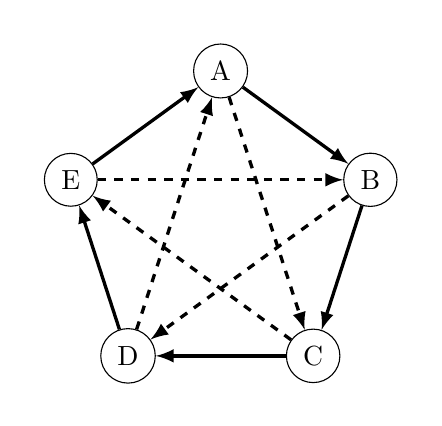
\begin{tikzpicture}
		\path (-2.45, -2.15) -- (-2.45, 2.55) -- (2.45, 2.55) -- (2.45, -2.15) -- cycle;
		\node[draw, circle]  (A) at (90:2) {A};
		\node[draw, circle]  (B) at (18:2) {B};
		\node[draw, circle]  (C) at (306:2) {C};
		\node[draw, circle]  (D) at (234:2) {D};
		\node[draw, circle]  (E) at (162:2) {E};
		\draw[very thick,  -latex] (A) to (B);
		\draw[very thick,  -latex] (B) to (C);
		\draw[very thick,  -latex] (C) to (D);
		\draw[very thick,  -latex] (D) to (E);
		\draw[very thick,  -latex] (E) to (A);
		
		\draw[very thick, dashed, -latex] (A) to (C);
		\draw[very thick, dashed, -latex] (B) to (D);
		\draw[very thick, dashed, -latex] (C) to (E);
		\draw[very thick, dashed, -latex] (D) to (A);
		\draw[very thick, dashed, -latex] (E) to (B);
		

	\end{tikzpicture}

\end{document}